\RequirePackage{luatex85}
\documentclass[tikz]{standalone}

\usepackage{pgfplots}
\pgfplotsset{compat=newest}
\usepgfplotslibrary{groupplots}
\usepgfplotslibrary{polar}
\usepgfplotslibrary{smithchart}
\usepgfplotslibrary{statistics}
\usepgfplotslibrary{dateplot}
\usepgfplotslibrary{ternary}

\usetikzlibrary{patterns}
\usepackage{xcolor}
\definecolor{cred}{HTML}{ED1C24}
\definecolor{cgrey}{HTML}{7F7F7F}
\definecolor{cblue}{HTML}{00A2E8}
\definecolor{cgreen}{HTML}{22B14C}
\definecolor{cyellow}{HTML}{FFF200}
\definecolor{corange}{HTML}{EA7904}
\definecolor{cpurple}{HTML}{9100FC}

\pgfplotsset{%
    discard if not/.style 2 args={%
        x filter/.code={%
            \edef\tempa{\thisrow{#1}}
            \edef\tempb{#2}
            \ifx\tempa\tempb
            \else
                \def\pgfmathresult{inf}
            \fi
        }
    }
}

\renewcommand{\familydefault}{\sfdefault}

\begin{document}
\begin{tikzpicture}
\begin{axis}[%
    height={5cm},
    width={7cm},
    xmin = -50,
    xmax = 850,
    xtick = {1, 200, 400, 600, 800},
    ytick = {0, 0.1, 0.2, 0.3, 0.4, 0.5, 0.6, 0.7, 0.8, 0.9, 1.0},
    yticklabels = {0, , , , , 0.5, , , , , 1},
    ymin = 0,
    %ymax = 1.1,
    xlabel = Ranked carbon AEFM indices (\#),
    ylabel = {Cumulative explained\\mass flow (0-99\%)},
    xlabel style = {font=\small},
    ylabel style = {font=\small,align=center},
    legend cell align = {left},
    xmajorgrids = {false},
    ymajorgrids = {false},
    xtick pos = bottom,
    ytick pos = left,
    legend style={font=\tiny},
    legend pos = south east,
    %title = {Glutamine},
    title style = {yshift=-1.5ex},
    axis line style={thick,black},
    xtick style={/pgfplots/on layer=axis foreground, thick, black},
    ytick style={/pgfplots/on layer=axis foreground, thick, black},
]
    \addplot[%
        scatter,
        mark=*, draw=black, line width=0.5pt, mark size=1pt,
        scatter src=explicit symbolic,
        scatter/classes={%
            1={mark=*,draw opacity=0, fill=cred}
        },
        each nth point=1,filter discard warning=false, unbounded coords=discard
    ] table [x=x, y=yc, meta=atom,discard if not={atom}{1}] {./cumulative-source-met-14.dat};
    \addplot[%
        scatter,
        mark=*, draw=black, line width=0.5pt, mark size=1pt,
        scatter src=explicit symbolic,
        scatter/classes={%
            2={mark=*,draw opacity=0, fill=cblue}
        },
        each nth point=1,filter discard warning=false, unbounded coords=discard
    ] table [x=x, y=yc, meta=atom,discard if not={atom}{2}] {./cumulative-source-met-14.dat};
    \addplot[%
        scatter,
        mark=*, draw=black, line width=0.5pt, mark size=1pt,
        scatter src=explicit symbolic,
        scatter/classes={%
            3={mark=*,draw opacity=0, fill=cgreen}
        },
        each nth point=1,filter discard warning=false, unbounded coords=discard
    ] table [x=x, y=yc, meta=atom,discard if not={atom}{3}] {./cumulative-source-met-14.dat};
    \addplot[%
        scatter,
        mark=*, draw=black, line width=0.5pt, mark size=1pt,
        scatter src=explicit symbolic,
        scatter/classes={%
            4={mark=*,draw opacity=0, fill=cyellow}
        },
        each nth point=1,filter discard warning=false, unbounded coords=discard
    ] table [x=x, y=yc, meta=atom,discard if not={atom}{4}] {./cumulative-source-met-14.dat};
    \addplot[%
        scatter,
        mark=*, draw=black, line width=0.5pt, mark size=1pt,
        scatter src=explicit symbolic,
        scatter/classes={%
            5={mark=*,draw opacity=0, fill=corange}
        },
        each nth point=1,filter discard warning=false, unbounded coords=discard
    ] table [x=x, y=yc, meta=atom,discard if not={atom}{5}] {./cumulative-source-met-14.dat};
    \addplot[%
        scatter,
        mark=*, draw=black, line width=0.5pt, mark size=1pt,
        scatter src=explicit symbolic,
        scatter/classes={%
            6={mark=*,draw opacity=0, fill=cpurple}
        },
        each nth point=1,filter discard warning=false, unbounded coords=discard
    ] table [x=x, y=yc, meta=atom,discard if not={atom}{6}] {./cumulative-source-met-14.dat};

    % Manually added
    \addplot[black, dashed, domain = -50:950,samples = 2] {0.99};
    \node[align=center,font=\small] at (rel axis cs:0.60,0.35) {Glutamine\\[0.25cm]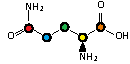
\includegraphics[width=3.0cm]{../../source-metabolite-structures/glutamine.pdf}};

\end{axis}
\end{tikzpicture}
\end{document}
